\documentclass{subfiles}
\begin{document}

Come si vede in \emph{Figura \ref{Fig:1.1}}, l'occhio umano ha una conformazione per lo più sferica.
Si circonda da quattro membrane: \emph{cornea \emph{e} sclera},che lo coprono dall'esterno, \emph{coroide \emph{e} retina}.

Circa la visione in se, questa è permessa da recettori luminosi posti sulla retina.
Tali recettori sono distinti per struttura e funzionalità, si hanno i \emph{bastoncelli \emph{e} coni}.\\

\begin{wrapfigure}[17]{l}{0.525 \textwidth}
    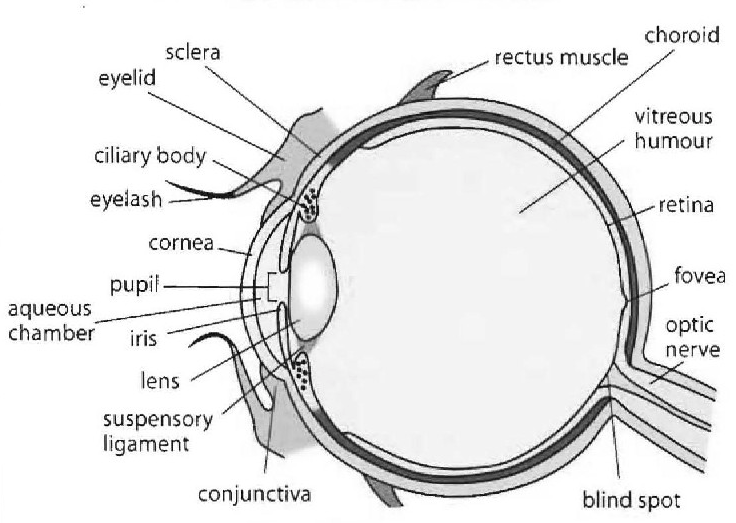
\includegraphics[scale = 0.4]{Images/Human Eye.png}
    \caption{Struttura dell'occhio umano.}
    \label{Fig:1.1}
\end{wrapfigure}

Analizzando le funzionalità dei due, i recettori conici sono disposti nella parte centrale dell'occhio, la \emph{fovea}, sono molto sensibili alle variazioni di colore,
e ciascun recettore è connesso ad un proprio terminale nervoso. Sono responsabili della visione \emph{fotopica}(visione a colori).
I bastoncelli, distribuiti su tutta la retina e soggetti alle variazioni luminose, connessi ad un terminale nervoso comune, hanno lo scopo di fornire un immagine generale.
Sono responsabili della visione \emph{scotopica}(visione a scala di grigi).

Osservando \emph{Figura \ref{Fig:1.1}}, si osserva che è presente una porzione dell'occhio, quella da cui di base si estende il nervo ottico,
che è priva di recettori: tale punto è detto \emph{blind spot}, proprio perché non contribuisce alla visione.
Si potrebbe pertanto pensare che la presenza di questo punto cieco, possa creare una sorta di vuoto nell'immagine.
Da un punto di vista tecnico, è così. Per quel che riguarda la visione, così non è: le informazioni carpite dagli occhi giungono al cervello passando per il \emph{chiasma},
essendo questi un ``canale'' comune, trasferisce in contemporanea informazioni di entrambi gli occhi, permettendo al cervello di ottenere un'immagine ``pulita''.

\begin{Remark*}
    la visione non è globale: ossia nella realtà dei fatti ad essere messa a fuoco non è l'intera scena, quanto più una piccola porzione della stessa,
    quella perpendicolare alla fovea per la precisione, la nitidezza del resto dell'immagine è dovuta al cervello.
\end{Remark*}

\subsection{Immagini digitali}
\subfile{Sotto Sezioni/Sottosezione 1.1 - Immagini digitali.tex}
\clearpage
\end{document}